\documentclass[hyperref={pdfpagelabels=false}]{beamer}
\mode<presentation>
{
  \usetheme{Warsaw}
}
\usepackage{multimedia}
\usepackage[english]{babel}
\usepackage[latin1]{inputenc}
\usepackage{times}
%\usepackage[T1]{fontenc}
%\usepackage{amsmath}
\usepackage{tikz}
\usepackage[retainorgcmds]{IEEEtrantools}

\newcommand{\bs}{\boldsymbol}
\newcommand{\ev}{\end{array}\right]}
\newcommand{\bv}{\left[\begin{array}{c}}
\newcommand{\bm}{\left[\begin{array}{ccc}}
\newcommand{\bmm}{\left[\begin{array}{cc}}
\newcommand{\tr}{\mathrm{T}}
\newcommand{\func}{\mathcal{F}}

\title[High-Fidelity Multiplysics Simulations]
% (optional, use only with long paper titles)
{High-Fidelity Multiplysics Simulations with Adaptive Mesh Refinement}

%\subtitle
%{\footnotesize (Diplomarbeit im Rahmen des Doppeldiploms \\ Universit\"at Karlsruhe (TH) / \\ Institut National Polytechnique de Grenoble)}

\author[D. Lebrun-Grandi\'e] % (optional, use only with lots of authors)
{Damien Lebrun-Grandi\'e\footnote{ \texttt{$<$\href{mailto:lebrungd@neo.tamu.edu}{lebrungd@neo.tamu.edu }$>$} }, Jean Ragusa}
%Nuclear Engineering Department \\
%Texas A\&M University}

\institute[Texas A\&M University] % (optional, but mostly needed)
{Nuclear Engineering Department \\ Texas A\&M University}

\date[MEPhI, Sep 2010] % (optional, should be abbreviation of conference name)
{Moscow Engineering Physics Institute \\ September 2010}
% - Either use conference name or its abbreviation.
% - Not really informative to the audience, more for people (including
%   yourself) who are reading the slides online

\subject{Nuclear Engineering and Numerical Methods}
% This is only inserted into the PDF information catalog. Can be left
% out. 



% If you have a file called "university-logo-filename.xxx", where xxx
% is a graphic format that can be processed by latex or pdflatex,
% resp., then you can add a logo as follows:

\pgfdeclareimage[height=1.5cm]{logo}{tamu-logo.png}
\logo{\pgfuseimage{logo}}

% Delete this, if you do not want the table of contents to pop up at
% the beginning of each subsection:
\AtBeginSubsection[]
{
  \begin{frame}<beamer>{Outline}
    \tableofcontents[currentsection,currentsubsection]
  \end{frame}
}
 
% If you wish to uncover everything in a step-wise fashion, uncomment
% the following command: 

%\beamerdefaultoverlayspecification{<+->}

\begin{document}

\begin{frame}
  \titlepage
\end{frame}

% Structuring a talk is a difficult task and the following structure
% may not be suitable. Here are some rules that apply for this
% solution: 

% - Exactly two or three sections (other than the summary).
% - At *most* three subsections per section.
% - Talk about 30s to 2min per frame. So there should be between about
%   15 and 30 frame ts, all told.

% - A conference audience is likely to know very little of what you
%   are going to talk about. So *simplify*!
% - In a 20min talk, getting the main ideas across is hard
%   enough. Leave out details, even if it means being less precise than
%   you think necessary.
% - If you omit details that are vital to the proof/implementation,
%   just say so once. Everybody will be happy with that.

% display outline using table of contents
\begin{frame}{Outline}
   \tableofcontents
%   \tableofcontents[hideallsubsections,pausesections]
  % You might wish to add the option [pausesections]
\end{frame}

\begin{frame}{Biography -- Education}

\begin{minipage}{5cm}
\scriptsize
\begin{tabular}{r|p{9.5cm}}
%TEXAS
\textsc{Current} & \textbf{Texas A\&M University} -- USA \\
\textsc{Jan 2010} & PhD at the Department of Nuclear Engineering \\
\multicolumn{2}{c}{} \\
%KARLSRUHE
\textsc{Oct 2007} & \textbf{University of Karlsruhe (TH)} -- Germany \\
\textsc{Dec 2009} & Master of Science (Diplom) in Physics \\
 & \tiny Thesis: ``Measurement and analysis of fast neutron and gamma-ray flux spectra in a neutronics mock-up of the European Helium-Cooled Lithium-Lead Test Blanket Module for ITER'' \\
\multicolumn{2}{c}{} \\
%GRENOBLE
\textsc{Sep 2005} & \textbf{Grenoble National Engineering School for Physics} -- France\\
\textsc{May 2007} & Master's Degree in Engineering (Dipl\^ome d'ing\'enieur) \\
& with specialty option ``Energy and Nuclear Engineering'' \\
& \tiny Leading French school in physics, part of the Grenoble Institute of Technology \\
\multicolumn{2}{c}{} \\
%BORDEAUX
\textsc{Sep 2003} & \textbf{Lyc\'ee Michel Montaigne in Bordeaux} -- France \\
\textsc{Jul 2005} & \tiny University level preparation in Mathematics, Physics and Chemistry for competitive entrance exams to French ``Grandes Ecoles'' \\
\end{tabular}
\end{minipage}

\end{frame}



\begin{frame}{Biography -- Work experience}

\begin{minipage}{5cm}
\scriptsize
\begin{tabular}{r|p{9.5cm}}
%\emph{Current} & Research Assistant, College Station \\
%\textsc{Jan 2010} & \emph{Texas A\&M University, Department of Nuclear Engineering} \\
%& \footnotesize{High-fidelity multiphysics simulations with hp-adaptivity.} \\
%\multicolumn{2}{c}{} \\ %this clears the space between two jobs
%DIPLOMARBEIT
\textsc{Feb 2009} & Trainee, Eggenstein-Leopoldshafen -- Germany\\
\textsc{Dec 2009} & \emph{\textbf{Institute for Neutron Physics and Reactor Technology}, Karlsruhe Institute of Technology} \\
%& \emph{Forschungszentrum Karlsruhe GmbH,} \\
& \tiny{Conducted an experiment aiming to validate the neutronics design of a Test Blanket System for the ITER fusion reactor.} \\
\multicolumn{2}{c}{} \\ %this clears the space between two jobs
%INL
\textsc{Sep 2008} & Trainee, Idaho Falls -- USA\\
\textsc{Dec 2008} & \emph{\textbf{Idaho National Laboratory}, US Department Of Energy} \\
& \tiny{Worked in a team on development of a parallel computational framework for coupled systems of nonlinear equations.} \\
\multicolumn{2}{c}{} \\ %this clears the space between two jobs
%EIfER
\textsc{Nov 2007} & Research Assistant, Karlsruhe -- Germany\\
\textsc{Jul 2008} & \emph{\textbf{European Institute for Energy Research}, joint research institute EDF/KIT} \\
& \tiny{Analysed data results of field experiments with fuel cell systems performed by French firm \'Electricit\'e de France.} \\
\multicolumn{2}{c}{} \\ %this clears the space between two jobs
%AUCKLAND
\textsc{Jun 2007} & Summer Internship -- New Zealand \\
\textsc{Aug 2007} & \emph{\textbf{Department of Physics}, University of Auckland} \\
& \tiny{Worked on a project deploying marine turbines for power generation in conjunction with company Energy Pacifica.} \\
\end{tabular}
\end{minipage}

\end{frame}

\begin{frame}{$hp$-FEM}
  {Definition}
  \tiny
  "The \alert{$hp$-FEM} is a general version of the finite element method (FEM), a numerical method for solving partial differential equations based on piecewise-polynomial approximations that employs elements of variable size ($h$) and polynomial degree ($p$).  The origins of $hp$-FEM date back to the pioneering work of Ivo Babuska who discovered that the finite element method \alert{converges exponentially fast when the mesh is refined using a suitable combination of $h$-refinements} (dividing elements into smaller ones) \alert{and $p$-refinements} (increasing their polynomial degree).  The exponential convergence makes the method a very attractive choice compared to most other finite element methods which only converge with an algebraic rate.  The exponential convergence of the $hp$-FEM was not only predicted theoretically but also observed by numerous independent researchers." [Wikipedia]

\end{frame}

\begin{frame}{$hp$-FEM}
  \footnotesize
  
  \begin{block}{Hermes Project}
Hermes is a C++ library for rapid development of $hp$-FEM solvers.  The library is currently developed by Pavel Solin's group at the University of Nevada, Reno (UNR), and their collaborators from numerous places around the globe.
  \end{block}
\vspace{.3cm}

Hermes provides
\begin{itemize}
\item mature $hp$-adaptivity algorithms
\item wide applicability
\item arbitrary level hanging nodes
\item multimesh $hp$-FEM
\end{itemize}

\end{frame}

%%%%%%%%%%%%%%%%%%%%%%%%%%%%%%%%%%%%%%%%%%%%%%%%

\begin{frame}{$hp$-FEM}
  {Understanding the convergence rates}
  
  \scriptsize

    When using elements of degree $ p $ we expect a slope of $ - p/d $ on the log-log scale
    
    ($ d $ is the dimension)

    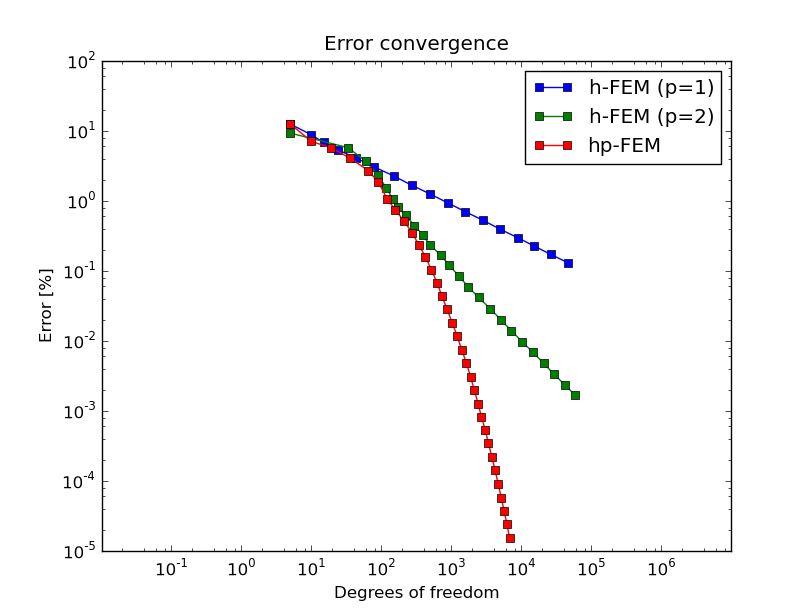
\includegraphics[width=6cm]{figures/conv_dof15}
    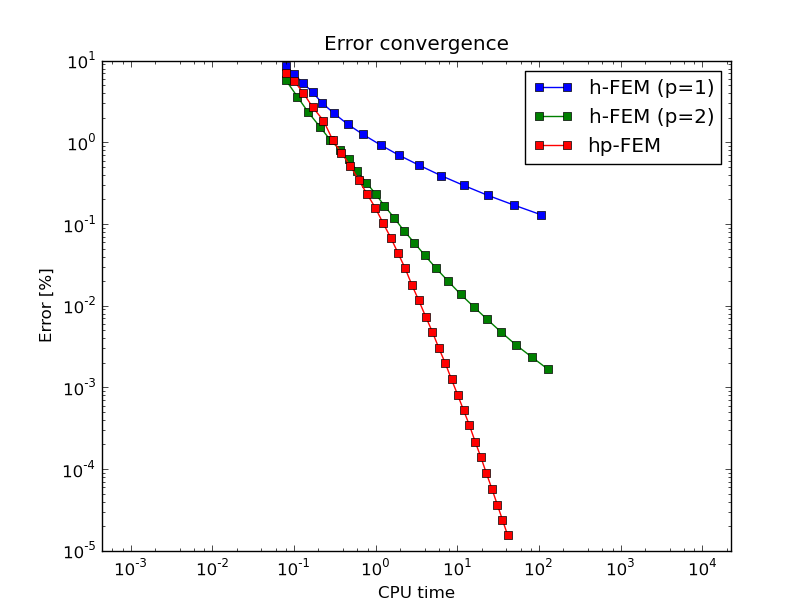
\includegraphics[width=6cm]{figures/conv_cpu15}
    

\end{frame}

%%%%%%%%%%%%%%%%%%%%%%%%%%%%%%%%%%%%%%%%%%%%%%%%

\begin{frame}{$hp$-FEM}
  {Adaptivity in the $hp$-FEM and in Hermes}
  
  \begin{columns}
  \begin{column}{5cm}
    \tiny
    An element can be refined in many different ways

     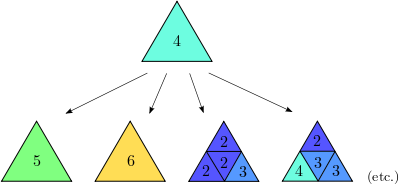
\includegraphics[width=5cm]{figures/refinements}
     
     \vspace{.3cm}
     
     Number of refinement candidates relatively low in $ h $ or $ p $ adaptivity, much higher in $ hp $ adaptivity
      
     %The number of possible element refinements is implementation-dependent.   In general it is very low in $ h $ or $ p $ adaptivity, much higher in $ hp $ adaptivity, and it rises even more when anisotropic refinements are enabled.

  \end{column}
  \begin{column}{7cm}
  \scriptsize  
  \begin{block}{Automatic adaptivity in Hermes}
    \begin{enumerate}
    \item Generate refinement candidates
    \item Estimates local errors by projecting reference solution onto FE spaces
    \item Calculate number of degree of freedom (DOF) contributed by each candidate
    \item Calculates a score for each candidate, and sort them according to their scores
    \item Select candidate with highest score
    \end{enumerate}
  \end{block}

    By default in Hermes, the score is $ s = \frac{\log_{10} e_{0} - \log_{10} e}{(d_{0} - d)^{\xi}} $
    %where $ e $ and $ d $ are an estimated error and an estimated number of DOF of a candidate respectively, $ e_0 $ and $ d_0 $ are an estimated error and an estimated number of DOF of the examined element respectively, and $ \xi $ is a convergence exponent
    
    %and the error estimate is calculated as $ e = \frac{\|u-u_{ref}\|_{H^{1}}}{\|u_{ref}\|_{H^{1}}} $

  \end{column}
  \end{columns}

\end{frame}



\begin{frame}{$hp$-FEM}
  {Multimesh}

   \tiny
   (A) is the master mesh, (B) - (D) three different meshes, and (E) is the virtual union mesh
    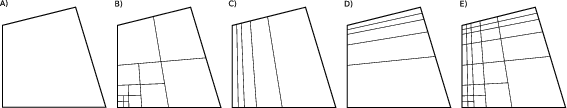
\includegraphics[width=8cm]{figures/multimesh}

    \vspace{.3cm}

    The union mesh is not constructed physically in the computer memory -- it merely serves as a "hint" to correctly transform integration points while integrating over sub-elements of the elements of the existing meshes

    %The following figure shows the integration over an element  of the virtual union mesh, and what are the appropriate subelements of the existing elements where this integration is performed
    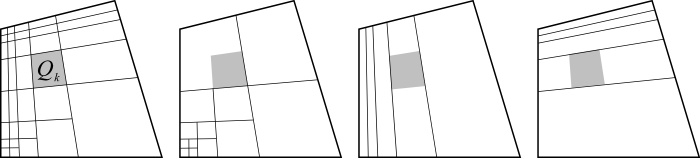
\includegraphics[width=8cm]{figures/multimesh2}

    %The adaptivity procedure for single PDE could be extended directly to systems of PDEs.  In this way, error estimates in $ H^{1} $ norm are calculated for elements in both spaces independently and the worst ones are refined. However, this approach is not optimal if the PDEs are coupled, since an error caused in one solution component influences the errors in other components and vice versa.

    %Recall that in elliptic problems the bilinear form $ a(u, v) $ defines the energetic inner product, $ (u, v)_{e} = a(u, v) $.

    %The norm induced by this product $ \|u\|_{e} = \sqrt{(u, u)_{e})} $, is called the energy norm. When measuring the error in the energy norm of the entire system, one can reduce the above-mentioned difficulties dramatically. When calculating the error on an element, the energy norm accounts also for the error caused by other solution components.

%The adaptivity algorithm does not make distinctions between various meshes. The elements of all meshes in the system are put into one single array, sorted according to their estimated errors, and then the ones with the largest error are refined. In other words, it may happen that all elements marked for refinement will belong just to one mesh.

\end{frame}

\begin{frame}{$hp$-FEM}
  {Example with Hermes2D}
  \tiny
  \begin{columns}
  \begin{column}{5cm}
    We consider a simplified Fitzhugh-Nagumo system
      
    $ -d_u^2 \Delta u - f(u) + \sigma v = g_1 $

    $ -d_v^2 \Delta v - u + v = g_2 $
    
    \vspace{.3cm}

    In the original equation, $ f(u) = \lambda u - u^3 - \kappa $.  For simplicity, here we just take $ f(u) = u $.

    Domain: Square $ (-1,1)^2 $.
    
    BC: Both solution components are zero on the boundary.
 

    %The following two figures show the solutions $ u $ and $ v $.  Notice their large qualitative differences: While $ u $ is smooth in the entire domain, $ v$ has a thin boundary layer along the boundary:
    \hspace{0.5cm} 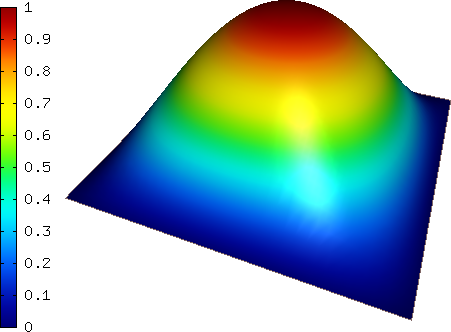
\includegraphics[width=3cm]{figures/solution_u}
    
    \hspace{1.5cm} 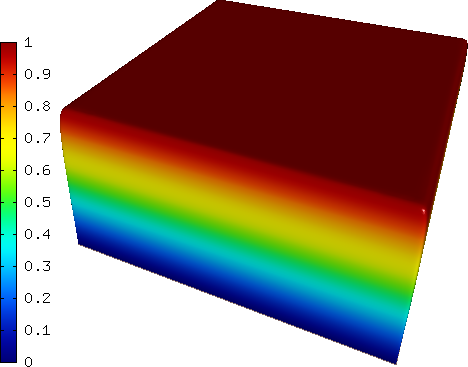
\includegraphics[width=3cm]{figures/solution_v}

  \end{column}
  \begin{column}{7cm}
     
    Exact solution: The functions $g_1$ and $g_2$ were calculated so that the exact solution is
    $ u(x,y) = \cos(\frac{\pi x}{2}) \cos(\frac{\pi y}{2}) $
    
    $ v(x,y) = \left[1 - \frac{(\exp(k x)+\exp(-k x))}{(\exp(k) + exp(-k)}\right] \left[1 - \frac{(\exp(k y)+\exp(-k y))}{(\exp(k) + exp(-k)}\right] $
  
    \vspace{.3cm}
  
    Resulting mesh for $ u $ and $ v $ obtained using conventional (single-mesh) hp-FEM: 12026 DOF (6013 for each solution)
    
    Resulting mesh for $ u $ obtained using the multimesh hp-FEM: 169 DOF
    
    Resulting mesh for $ v $ obtained using the multimesh hp-FEM: 3565 DOF
    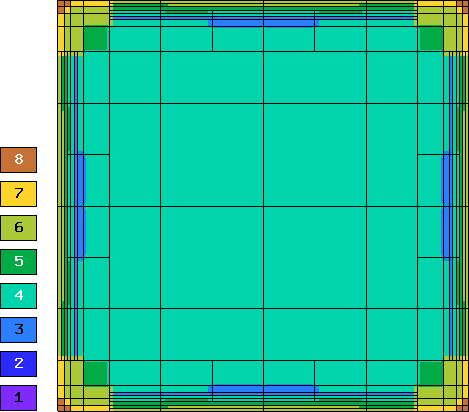
\includegraphics[width=2.3cm]{figures/mesh_single}
    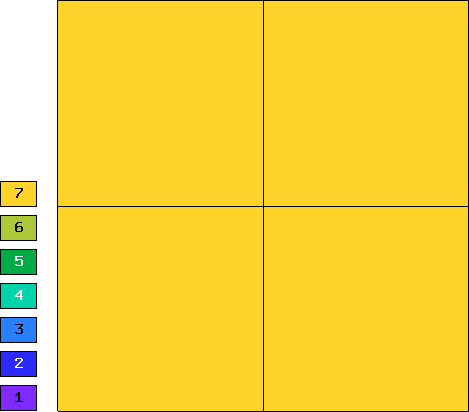
\includegraphics[width=2.3cm]{figures/mesh_multi_u}
    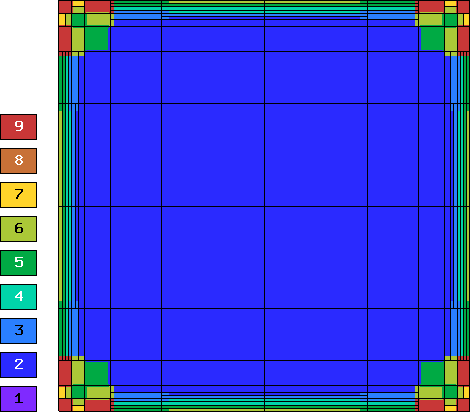
\includegraphics[width=2.3cm]{figures/mesh_multi_v}

    DOF and CPU convergence graphs:
    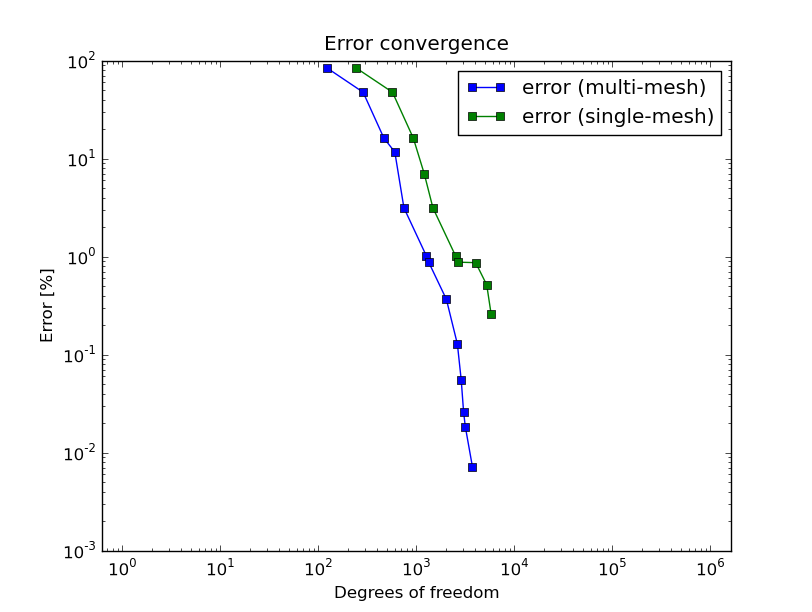
\includegraphics[width=3.5cm]{figures/conv_dof12}
    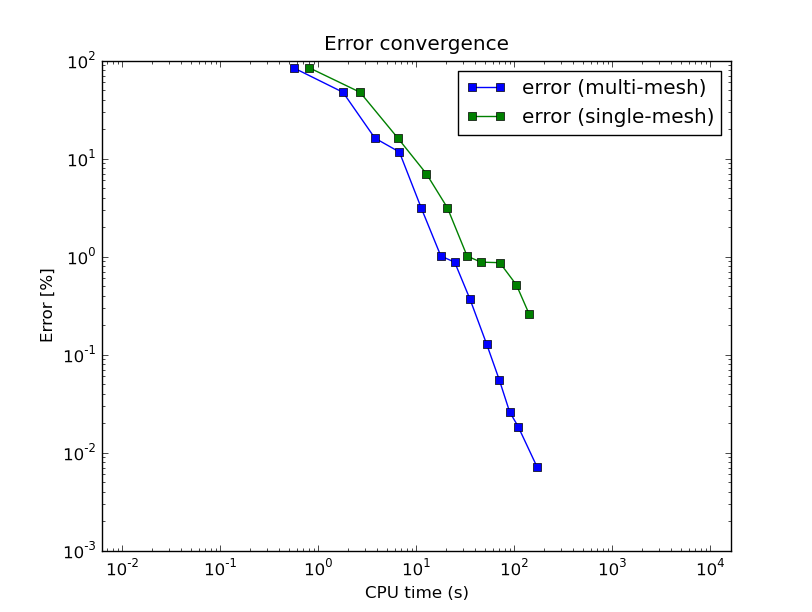
\includegraphics[width=3.5cm]{figures/conv_cpu12}
    
  \end{column}
  \end{columns}

\end{frame}


%%%%%%%%%%%%%%%%%%%%%%%%%%%%%%%%%%%%%%%%%%%%%%%%%%%%%%%%%%%%%%%%%%%%%%%%%%%
%%% ADJOINT EQUATIONS


\begin{frame}{Nonlinear Adjoint Sensitivity Analysis}
  {Elements of theory on the adjoint}
  \tiny

  \begin{columns}[T]
  \begin{column}{5.5cm}

  \begin{block}{Generic coupled physics problem}
    We consider nonlinear system of $ N_{u} $ equations together with initial and boundary conditions
    \begin{align}
      \begin{cases}
      A \bs{u} = \bs{f} & \bs{x} \in \Omega , t_{init} < t < t_{final} \\
      \bs{u} = \bs{u}_{init} & \bs{x} \in \Omega , t = t_{init} \\
      B \bs{u} = \bs{u}_{\Gamma} & \bs{x} \in \Gamma , t_{init} < t < t_{final}
      \end{cases} \label{system_eq}
    \end{align}
  \end{block}

    $ A $, $ \bs{f} $, $ \bs{u}_{init} $, B, and $ \bs{u}_{\Gamma} $ depend on a parameter $ \bs{p} $ of dimension $ N_{p} $
    
    $ A $ and $ B $ may depend on the solution $ \bs{u} $

  \begin{block}{Functional of the solution}
    We compute a functional $ \func $ of the solution $ \bs{u} $ of \eqref{system_eq}
    \begin{align}
      \func (\bs{u})
      = ( \bs{\sigma}, \bs{u} ) \nonumber
    \end{align}
  \end{block}

    $ (., .) $ represents some ``scalar'' product that I do not want to define here...

    $ \bs{\sigma} $ is a weighting function associated to $ \func $ (e.g. response of a detector)
    
    \vspace{.3cm}
     
    We assume that the parameter $ \bs{p} $ is perturbed by $ \bs{\delta p} $, i.e. instead of $ \bs{p} $, we have now 
    $ \bs{p} + \bs{\delta p} $
    
  \end{column}
  \begin{column}{5.5cm}
    
   How is $ \func $ affected by the change in $ \bs{p} $?
    
    \vspace{.3cm}
    
    We define an adjoint operator $ A^{*} $ that verifes
    %\begin{align}
    $  ( \bs{u}^{*}, A \bs{u} ) = ( A^{*} \bs{u}^{*}, \bs{u} ) \label{duality}$
    %\end{align}
    (or at least we would like him to do so...)
    
  \begin{block}{Adjoint}
    At this point, we define the following problem that is said to be "adjoint" of \eqref{system_eq}
    \begin{align}
      \begin{cases}
      A^{*} \bs{u}^{*} = \bs{\sigma} & \bs{x} \in \Omega , t_{init} < t < t_{final} \\
      \bs{u}^{*} = \bs{u}^{*}_{final} & \bs{x} \in \Omega , t = t_{final} \\
      B^{*} \bs{u}^{*} = \bs{u}^{*}_{\Gamma} & \bs{x} \in \Gamma , t_{init} < t < t_{final}
      \end{cases} \label{adjoint_eq}
    \end{align}
  \end{block}
    Remark: Note that $ A ^{*} $ and $ B^{*} $ depend on $ \bs{u} $
        
    \vspace{.3cm}
    
    The duality relation between the solutions of \eqref{system_eq} and \eqref{adjoint_eq} reads
    
    \begin{center} \small \alert {
    \begin{tabular}{|c|} \hline $ ( \sigma, \bs{\delta u} ) = ( \bs{u}^{*}, \bs{\delta f} ) - ( \bs{u}^{*}, (\delta A) \bs{u} ) $ \\ \hline \end{tabular}
    } \end{center}

    Why is that advantageous?
    
  \end{column}
  \end{columns}

\end{frame}


%%%%%%%%%%%%%%%%%%%%%%%%%%%%%%%%%%%%%%%%%%%%%%%%%%%%%%%%%%%%%%%%%%%%%%%%%%%
%%% PERTURBATION THEORY

\begin{frame}{Nonlinear Adjoint Sensitivity Analysis}
  {Analysis of a coupled neutronics/thermal-hydaulics problem}

  \begin{columns}[T]
    \begin{column}{5cm}
    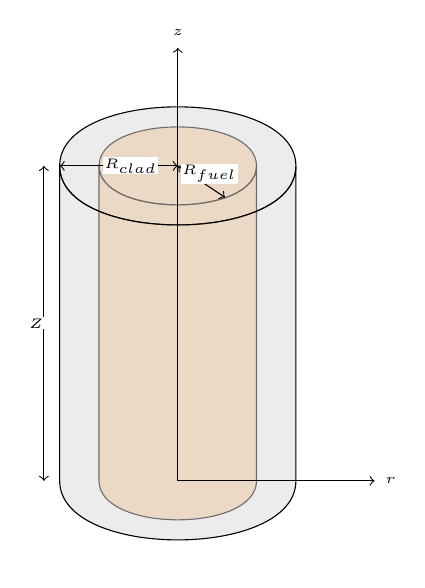
\begin{tikzpicture}

    \tikzstyle{ann} = [fill=white, font=\tiny, inner sep=.5pt]

    % Fuel
    \draw[fill=orange!60, fill opacity=0.5] (0.5,0) to
        [controls=+(90:0.66) and +(90:0.66)] (2.5,0);

    \draw[fill=orange!60, fill opacity=0.5] (0.5,0) .. controls +(-90:0.66)
    and +(-90:0.66) .. (2.5,0);

    \draw[fill=orange!60, fill opacity=0.5] (0.5,0) .. controls +(-90:0.66)
    and +(-90:0.66) .. (2.5,0)
        -- (2.5,-4) .. controls +(-90:0.66) and +(-90:0.66) .. (0.5,-4) -- (0.5,0);


    % Clad
    \draw[fill=lightgray!60, fill opacity=0.5] (0,0) to
        [controls=+(90:1.0) and +(90:1.0)] (3,0);

    \draw[fill=lightgray!60, fill opacity=0.5] (0,0) .. controls +(-90:1.0)
    and +(-90:1.0) .. (3,0);

    \draw[fill=lightgray!60, fill opacity=0.5] (0,0) .. controls +(-90:1.0)
    and +(-90:1.0) .. (3,0)
        -- (3,-4) .. controls +(-90:1.0) and +(-90:1.0) .. (0,-4) -- (0,0);

    % Rfuel and Rclad
    \draw[arrows=<->,line width=.4pt](1.5,0)--(2.1,-.4);
    \draw[arrows=<->,line width=.4pt](1.5,0)--(0,0);
    \node[ann] at (0.9,0) {$R_{clad}$};
    \node[ann] at (1.9,-0.1) {$R_{fuel}$};

    \draw[arrows=<->,line width=.4pt](-0.2,0)--(-0.2,-4);
    \node[ann] at (-0.3,-2) {$Z$};

    % z- and r- axes
    \draw[arrows=->,line width=.4pt](1.5,-4)--(1.5,1.5);
    \draw[arrows=->,line width=.4pt](1.5,-4)--(4.0,-4.0);
    \node[ann] at (1.5,1.7) {$z$};
    \node[ann] at (4.2,-4) {$r$};

    %\node[ann] at (3.5,0.5) {$\Phi=0\mbox{ at }z=Z$};
    %\node[ann] at (3.5,-4.5) {$\Phi=0\mbox{ at }z=0$};

    %\node[ann] at (5.5,-1.3) {$-k_{clad}\nabla T^{clad}
    %                         =h_{conv}(T^{clad}-T_{m})
    %                         \mbox{ at }r=R_{clad}$};
    %\node[ann] at (4.3,-2.8) {$-k_{fuel}\nabla T^{fuel}
    %                           =-k_{clad}\nabla T^{clad}
    %                           =h_{gap}(T^{fuel}-T^{clad})
    %                           \mbox{ at }r=R_{fuel}$};

    %\node[ann] at (3.5,-4.7) {$H=0\mbox{ at }z=0$};

\end{tikzpicture}


  \end{column}

  \begin{column}{7cm}
    \tiny

    \begin{block}{Neutronics - multigroup diffusion equation}
      \begin{align}
        \left( \frac{1}{v^{g}} \partial_{t} 
        - \nabla \cdot D^{g} \nabla
        + \Sigma_{r}^{g} \right) \Phi^{g}
        = \frac{1}{\lambda} \chi^{g} \sum_{g'} \nu \Sigma_{f}^{g'} \Phi^{g'}
        + \sum_{g'\neq g} \Sigma_{s}^{g' \rightarrow g} \Phi^{g'}
        \nonumber 
      \end{align}
    \end{block}

    \begin{block}{Heat transfer  - heat conduction equation}
      \begin{align}
        \left( \rho C_{p} \partial_{t}
        - \nabla \cdot k \nabla \right) T 
        = q''' \nonumber
      \end{align}
    \end{block}
 
    \begin{block}{Fluid dynamics  - enthalpy balance}
      \begin{align}
        \left( \partial_{t}
        - \nabla \cdot \bs{u} \right) \rho_m H 
        = - \nabla \varphi \nonumber
      \end{align}
    \end{block}

  \end{column}
  \end{columns}

\end{frame}




%%%%%%%%%%%%%%%%%%%%%%%%%%%%%%%%%%%%%%%%%%%%%%%%%%%%%%%%%%%%%%%%%%%%%%%%%%%
%%% NEUTRONICS

\begin{frame}{Equations for the model - Neutronics}

  \tiny

  \begin{columns}[T]
  \begin{column}{7cm}

    For the neutron field we use:

    \begin{block}{1D two-group neutron diffusion equations}
      \begin{align}
        \frac{1}{v^{1}} \partial_{t} \Phi^{1} 
        - \partial_{z} \left( D^{1} \partial_{z} \Phi^{1} \right) 
        + \Sigma_{r}^{1} \Phi^{1}
        - \frac{1}{\lambda} \nu \Sigma_{f}^{1} \Phi^{1}
        - \frac{1}{\lambda} \nu \Sigma_{f}^{2} \Phi^{2}
        & = 0 \nonumber \\
        \frac{1}{v^{2}} \partial_{t} \Phi^{2} 
        - \partial_{z} \left( D^{2} \partial_{z} \Phi^{2} \right) 
        + \Sigma_{r}^{2} \Phi^{2}
        - \Sigma_{s}^{1 \rightarrow 2} \Phi^{1}
        & = 0 \nonumber
      \end{align}
    \end{block}

    Neutron flux in group $ g $: $ \Phi^{g} = \Phi^{g}(t,z) $
    
    We denote "1" the fast and "2" the thermal groups.

    \begin{block}{Vacuum boundary conditions}
      \begin{align}
        \Phi^{g} = 0 
        \quad \mbox{at } z = 0, Z \nonumber
      \end{align}
    \end{block}

  \end{column}

  \begin{column}{5cm}

    Model assumptions:
    \begin{itemize}
    \item no dependence of the neutron field on the $ r $ coordinate $ \Rightarrow $ $ \nabla \cdot D^{g} \nabla \rightarrow \partial_{z} D^{g} \partial_{z} $
    \item only two energy groups: $ g = 1, 2 $
    \item all fission neutrons will be born in the fast group: $ \chi^{1} = 1 $ and $ \chi^{2} = 0 $
    \item no upscattering: $ \Sigma_{s}^{2\rightarrow 1} = 0 $
    \end{itemize}
 
    \vspace{.5cm}

    The cross sections and the diffusion coefficients are functions of the moderator density $ \rho_{m} $ and the temperature $ T_{eff} $ defined as:
    \begin{align}
      T_{eff} = 
      \alpha \left. T(t,z,r) \right|_{r=0} 
      + (1-\alpha) \left. T(t,z,r) \right|_{r=R_{fuel}} \nonumber
    \end{align}
    (A closure relation gives $ \rho_{m} $ as a function of the enthalpy $ H $ and the pression $ P $)

  \end{column}
  \end{columns}

\end{frame}


%%%%%%%%%%%%%%%%%%%%%%%%%%%%%%%%%%%%%%%%%%%%%%%%%%%%%%%%%%%%%%%%%%%%%%%%%%%
%%% HEAT TRANSFER

\begin{frame}{Equations for the model - Fuel pin heat transfer}

  \tiny

  \begin{columns}
  \begin{column}{8cm}

    For the fuel pin heat transfer, we consider:

    \begin{block}{Heat conduction equations through fuel pin and cladding}
      \begin{align}
        \rho_{fuel} C_{p}^{fuel} \partial_{t} T^{fuel} 
        - (1/r) \partial_{r} r\ k_{fuel} \partial_{r} T^{fuel} 
        = \sum_{g} \kappa^{g} \Sigma_{f}^{g} \Phi^{g}
        \quad &\mbox{for } 0 < r < R_{fuel} \nonumber \\
        \rho_{clad} C_{p}^{clad} \partial_{t} T^{clad} 
        - (1/r) \partial_{r} r\ k_{clad} \partial_{r} T^{clad} 
        = 0 \quad &\mbox{for } R_{fuel} < r < R_{clad} \nonumber
      \end{align}
    \end{block}

    Temperature in the pin fuel and cladding: $ T = T(t,z,r) $ 

%    Thus $ - k \nabla T \rightarrow - k \partial_{r} T $ and
%    $ \nabla \cdot k \nabla \rightarrow (1/r) \partial_{r} r\ k \partial_{r} $.

    \begin{block}{Heat flux from clad to coolant}
      \begin{align}
        -k_{clad} \partial_r T^{clad} = 
        h_{conv} \left( T^{clad} - T_{m} \right)
        \quad &\mbox{at } r = R_{clad} \nonumber
      \end{align}
    \end{block}

      Conductance of the gap between fuel and cladding is taken into account in the model through:
      \begin{align}
        -k_{fuel} \partial_{r} T^{fuel} =
        -k_{clad} \partial_{r} T^{clad} = 
        h_{gap} \left( T^{fuel} - T^{clad} \right)
        \quad &\mbox{at } r = R_{fuel} \nonumber 
      \end{align}

  \end{column}

  \begin{column}{4cm}

    Model assumption:
    \begin{itemize}
    \item no heat conduction along $ z $ axis 
    \item infinitely small gap between fuel and cladding
    \end{itemize}

    \vspace{.5cm}

    Thermal conductivity $ k $, heat capacity $ C_p $, and density $ \rho $, depend on the temperature itself $ \Rightarrow $ nonlinearity

    \vspace{.5cm}

%    In the source term, $ \kappa^{g} $ is the energy released per fission.

  \end{column}
  \end{columns}

\end{frame}


%%%%%%%%%%%%%%%%%%%%%%%%%%%%%%%%%%%%%%%%%%%%%%%%%%%%%%%%%%%%%%%%%%%%%%%%%%%
%%% FLUID DYNAMICS

\begin{frame}{Equations for the model - Fluid flow}

  \tiny

  \begin{columns}
  \begin{column}{8cm}

    For the coolant we use:

    \begin{block}{Enthalpy balance}
      \begin{align}
        \left[ \partial_{t} \rho_{m} 
        + \rho_{m} v \partial_{z} \right] H\ S_{h}
        = - k^{clad} \partial_{r} T (R_{clad}) \Delta z\ 2 \pi R_{clad} \nonumber
      \end{align}
    \end{block}

    Enthalpy of the coolant per unit mass: $ H = H(t,z) $

    \begin{block}{Inlet enthalpy}
      \begin{align}
        H = H_{in} \quad \mbox{at } z = 0 \nonumber
      \end{align}
    \end{block}

  Heat flux from the fuel pin: $ - k^{clad} \partial_{r} T (R_{clad}) = h_{conv} \left( T (R_{clad}) - T_{m} \right) $
  \end{column}

  \begin{column}{4cm}

    Model assumptions:
    \begin{itemize}
    \item pression $ P $ is fixed (155 bars)
    \item fluid flows along $z$-axis
    \item constant mass flow rate $ (\rho_{m} v) S_{h} $
    \end{itemize}

    \vspace{.5cm}

    There is a one-to-one relationship between $ \rho_{m} $, $ T_{m} $ and $ H $

  \end{column}
  \end{columns}

\end{frame}


%%%%%%%%%%%%%%%%%%%%%%%%%%%%%%%%%%%%%%%%%%%%%%%%%%%%%%%%%%%%%%%%%%%%%%%%%%%
%%% SOLVER

\begin{frame}{Newton's method equation solver}

  \tiny

  \begin{columns}
  \begin{column}{9cm}
    Let $ \bs{u} = \bv \Phi\\ T\\  H\\ \ev $ be the vector of unknown coefficients.

  \begin{block}{Newton's method}
    We put the nonlinear problem under the form:
    $
      \bs{r} ( \bs{u} ) = 0 \nonumber
    $,
    where $ \bs{r} $ is a nonlinear residual vector that we want to minimize.

    We take an initial ``guess'' $ \bs{u_{0}} $ and we iterate over $ k $ until $ \bs{r} (\bs{u_{k+1}} ) $ is sufficiently close to the zero vector:
    \begin{align}
      \bs{u}_{k+1} = \bs{u}_{k} 
      - \bs{J}^{-1}(\bs{u}_{k}) \bs{r}(\bs{u}_{k}) \nonumber
    \end{align}
    Here the $ J^{-1} $ is the inverse of the jacobian matrix

    $ J (\bs{u}) = D\bs{r} / D\bs{u} $ (= matrix of all 1st-order partial derivatives of the residual $ \bs{r} $ with respect to the vector of unknown $ \bs{u} $)

  \end{block}

    Remark: Newton's method will converge in one iteration for a linear problem.

  \end{column}
  \begin{column}{3cm}

    \hspace{.5cm}
    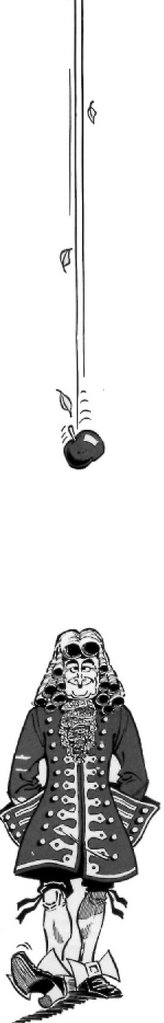
\includegraphics[width=1cm]{figures/newton}

  \end{column}
  \end{columns}

\end{frame}


\begin{frame}{}
  \Large
  \begin{columns}
  \begin{column}{7cm}
    \centering
    Questions ???
  \end{column}
  \begin{column}{5cm}
    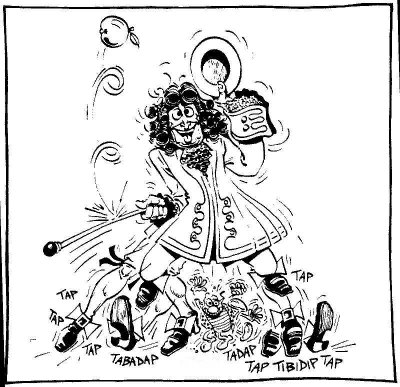
\includegraphics[width=4cm]{figures/newton_danse_by_gotlib}
  \end{column}
  \end{columns}
\end{frame}


%\begin{frame}{Bibliography}
%  \footnotesize
%  \bibliographystyle{ans}
%  \bibliography{thebibliography}
%\end{frame}



\end{document}


